% !TEX program = pdflatex
% Lunar-V2 / TSUKIMI --- Pipeline Roadmap (Developer Manual)
% Compile on Overleaf or locally with:
%   latexmk -pdf main.tex
% or:
%   pdflatex main && bibtex main && pdflatex main && pdflatex main

\documentclass[11pt,a4paper,openany,oneside]{book}
% ---------------------------------------------------------------------------
% Lunar-V2 / TSUKIMI  --  preamble.tex
% Overleaf-safe.  No shell-escape, no minted, no external tooling required.
% ---------------------------------------------------------------------------

% --- Core typesetting ------------------------------------------------------
\usepackage[utf8]{inputenc}
\usepackage[T1]{fontenc}
\usepackage{lmodern}
\usepackage[english]{babel}
\usepackage{microtype}
\usepackage[a4paper,margin=2.7cm,bindingoffset=0.3cm]{geometry}
\usepackage{setspace}
\onehalfspacing

% --- Math ------------------------------------------------------------------
\usepackage{amsmath,amssymb,amsthm,mathtools}
\usepackage{bm}
\usepackage{siunitx}
\sisetup{
  detect-all            = true,
  per-mode              = symbol,
  inter-unit-product    = \ensuremath{\cdot}
}

% --- Graphics --------------------------------------------------------------
\usepackage{graphicx}
\usepackage{subcaption}
\usepackage{float}
% Figures live in output/figures/ at the repo root.  Both paths are tried so
% the same preamble works (a) locally from docs/roadmap/ and (b) on Overleaf
% after flattening the figures into docs/roadmap/figures/.
\graphicspath{%
  {../../output/figures/}%
  {./figures/}%
  {figures/}%
}

% --- Tables ----------------------------------------------------------------
\usepackage{booktabs}
\usepackage{array}
\usepackage{longtable}
\usepackage{multirow}
\usepackage{tabularx}
\newcolumntype{Y}{>{\raggedright\arraybackslash}X}

% --- Colour & callouts ------------------------------------------------------
\usepackage{xcolor}
\definecolor{codegreen}{rgb}{0.0,0.45,0.0}
\definecolor{codegray}{rgb}{0.45,0.45,0.45}
\definecolor{codepurple}{rgb}{0.58,0.00,0.82}
\definecolor{codebg}{rgb}{0.97,0.97,0.97}
\definecolor{noveltyOrange}{HTML}{D97706}
\definecolor{warningRed}{HTML}{B91C1C}
\definecolor{milestoneGreen}{HTML}{047857}
\definecolor{conceptBlue}{HTML}{1D4ED8}

\usepackage[most]{tcolorbox}
\tcbuselibrary{skins,breakable}

\newtcolorbox{novelty}[1][]{%
  enhanced, breakable, sharp corners=downhill,
  colback=yellow!6, colframe=noveltyOrange,
  title=Research Novelty,
  fonttitle=\bfseries\sffamily,
  boxrule=0.8pt, left=4mm, right=4mm,
  #1%
}
\newtcolorbox{warning}[1][]{%
  enhanced, breakable, sharp corners=downhill,
  colback=red!4, colframe=warningRed,
  title=Warning,
  fonttitle=\bfseries\sffamily,
  boxrule=0.8pt, left=4mm, right=4mm,
  #1%
}
\newtcolorbox{milestone}[1][]{%
  enhanced, breakable, sharp corners=downhill,
  colback=green!4, colframe=milestoneGreen,
  title=Milestone,
  fonttitle=\bfseries\sffamily,
  boxrule=0.8pt, left=4mm, right=4mm,
  #1%
}
\newtcolorbox{concept}[1][]{%
  enhanced, breakable, sharp corners=downhill,
  colback=blue!4, colframe=conceptBlue,
  title=Concept,
  fonttitle=\bfseries\sffamily,
  boxrule=0.8pt, left=4mm, right=4mm,
  #1%
}

% --- Code listings ---------------------------------------------------------
\usepackage{listings}

\lstdefinestyle{pythonstyle}{%
  language=Python,
  backgroundcolor=\color{codebg},
  commentstyle=\color{codegreen}\itshape,
  keywordstyle=\color{blue!70!black}\bfseries,
  numberstyle=\tiny\color{codegray},
  stringstyle=\color{codepurple},
  basicstyle=\ttfamily\footnotesize,
  breakatwhitespace=false,
  breaklines=true,
  captionpos=b,
  keepspaces=true,
  numbers=left,
  numbersep=6pt,
  showspaces=false,
  showstringspaces=false,
  showtabs=false,
  tabsize=4,
  frame=single,
  rulecolor=\color{codegray!60},
  framesep=3pt,
  xleftmargin=12pt,
  xrightmargin=2pt,
  aboveskip=1.0em,
  belowskip=1.0em,
}
\lstset{style=pythonstyle}

% --- TikZ for flowcharts ---------------------------------------------------
\usepackage{tikz}
\usetikzlibrary{positioning,arrows.meta,shapes.geometric,calc,fit,backgrounds}

\tikzset{%
  phaseBlock/.style={
    rectangle, rounded corners=2mm, draw=black!70,
    minimum width=3.0cm, minimum height=1.1cm, align=center,
    font=\small\sffamily, fill=white},
  doneBlock/.style   ={phaseBlock, fill=green!12,  draw=milestoneGreen},
  activeBlock/.style ={phaseBlock, fill=yellow!18, draw=noveltyOrange},
  plannedBlock/.style={phaseBlock, fill=gray!10,   draw=black!60, dashed},
  arrowThick/.style={-{Stealth[length=3mm]}, thick, black!70},
}

% --- Hyperlinks & references -----------------------------------------------
\usepackage[colorlinks=true,
            linkcolor=blue!55!black,
            citecolor=green!40!black,
            urlcolor=cyan!60!black,
            bookmarksnumbered=true]{hyperref}
\usepackage[capitalise,noabbrev]{cleveref}

% --- Bibliography ----------------------------------------------------------
\usepackage[numbers,sort&compress]{natbib}
\usepackage{bibentry}

% --- Page style ------------------------------------------------------------
\usepackage{fancyhdr}
\pagestyle{fancy}
\fancyhf{}
\renewcommand{\chaptermark}[1]{\markboth{\thechapter.\ #1}{}}
\renewcommand{\sectionmark}[1]{\markright{\thesection\ #1}{}}
\fancyhead[LE,RO]{\thepage}
\fancyhead[LO]{\nouppercase\rightmark}
\fancyhead[RE]{\nouppercase\leftmark}
\renewcommand{\headrulewidth}{0.4pt}

% --- Chapter style ---------------------------------------------------------
\usepackage{titlesec}
\titleformat{\chapter}[display]
  {\normalfont\Huge\bfseries\sffamily}
  {\filleft\textcolor{black!40}{\fontsize{64}{74}\selectfont\thechapter}}
  {-0.3ex}
  {\titlerule[1pt]\vspace{1ex}\raggedright}
  [\vspace{0.4ex}\titlerule]
\titlespacing*{\chapter}{0pt}{-30pt}{30pt}

% --- Utility macros --------------------------------------------------------
\newcommand{\code}[1]{\texttt{\small #1}}
\newcommand{\repo}{\href{https://github.com/rp3gregorio/Lunar-V2}{\code{rp3gregorio/Lunar-V2}}}
\newcommand{\branch}{\code{claude/thermal-lunar-profile-repo-ZF4Mm}}

% Physical symbols used repeatedly
\newcommand{\Tsurf}{T_{\mathrm{surf}}}
\newcommand{\Tsub}{T_{\mathrm{sub}}}
\newcommand{\Kreg}{k_{\mathrm{reg}}}
\newcommand{\Kice}{k_{\mathrm{ice}}}
\newcommand{\Ksurf}{K_{s}}
\newcommand{\Kdeep}{K_{d}}
\newcommand{\Hscale}{H}
\newcommand{\Qb}{Q_{b}}
\newcommand{\Rsolar}{S_{\odot}}


\title{
  \vspace{-1.5cm}
  {\LARGE\bfseries Lunar-V2 / TSUKIMI Pipeline}\\[0.5em]
  {\Large A Developer's Manual and Scientific Roadmap}\\[0.3em]
  {\large Phase 1 through Phase 4}\\[1em]
  \rule{0.8\linewidth}{0.5pt}
}
\author{%
  Ramon III P.\ Gregorio\\[0.3em]
  \small Kasai Laboratory\\
  \small Department of Earth and Planetary Sciences\\
  \small Institute of Science Tokyo\\[0.5em]
  \small \texttt{rp3gregorio@gmail.com}
}
\date{Last revision: \today}

\begin{document}

\frontmatter
\maketitle

\begin{center}
\vspace*{2cm}
\begin{minipage}{0.85\linewidth}
{\large\bfseries\sffamily Abstract}\par\vspace{0.6em}
\noindent This manual documents the \textbf{TSUKIMI} (Thermal Subsurface
Understanding through Kinetic Ice Modeling and Illumination) pipeline
developed for the \texttt{Lunar-V2} code base. It bundles, in a single
volume, the numerical theory, implementation details, validation
results, and forward roadmap of a four-phase research program
culminating in a peer-reviewed manuscript for \textit{The Planetary
Science Journal} (PSJ) and a doctoral dissertation chapter at the
Institute of Science Tokyo.  The originality of this work lies at the
intersection of four ideas that have --- to the author's knowledge ---
never been combined in a single open-source lunar thermal pipeline:
(i) blind multi-site validation against every in-situ subsurface
thermal record currently available in the literature;
(ii) an ice-coupled conductivity feedback that closes the regolith
thermal budget self-consistently with the Klinger
($K_{\mathrm{ice}}=567/T$) law;
(iii) topographic slope correction applied at the pixel level, which
collapses the 40~K surface-temperature bias observed in the flat-surface
ChaSTE geometry; and
(iv) an end-to-end reproducible workflow in which every notebook
auto-installs its dependencies and auto-fetches its data from NASA/PDS
and NAIF.
\end{minipage}
\end{center}

\vfill
\begin{center}
\small
\fbox{
\begin{minipage}{0.9\linewidth}
\textbf{How to read this book.}\;
Chapters are organised by mission phase.  Each chapter opens with a
concise statement of goal and success criterion, proceeds to the
numerical theory and implementation, and closes with results or
deliverables and a bridge to the next phase.  The four thematic call-out
boxes (\emph{Concept}, \emph{Novelty}, \emph{Milestone}, \emph{Warning})
highlight ideas that the reader may want to bookmark.  Code listings
correspond to the \texttt{main} branch of
\url{https://github.com/rp3gregorio/Lunar-V2} at the date above.
\end{minipage}
}
\end{center}

\cleardoublepage
\tableofcontents
\cleardoublepage
\listoffigures
\cleardoublepage
\listoftables

\mainmatter

\chapter{Introduction}
\label{chap:introduction}

\section{Context: why lunar subsurface thermal models still matter}

Sixty years after the first Surveyor landers, the Moon's thermal
environment remains the single most important \emph{boundary condition}
for every volatile-stability, in-situ-resource-utilisation (ISRU), and
permanently shadowed region (PSR) study in the run-up to the Artemis
programme.  The Diviner radiometer on the Lunar Reconnaissance Orbiter
(LRO) has mapped top-of-regolith bolometric temperatures at
\SI{237}{\meter} pixel scale, but the \emph{subsurface} is
intrinsically opaque: we see it only through the handful of in-situ
probes emplaced by Apollo~15/17, Chang'E-4, and Chandrayaan-3's ChaSTE
instrument.

Every published lunar thermal model must therefore survive the same
four sanity checks:
\begin{enumerate}
  \item does it reproduce the Apollo HFE deep-sensor equilibrium
        temperatures ($\sim$\SI{250}{\kelvin}) at each site?
  \item does it recover the diurnal surface-temperature amplitude
        observed by Diviner and Chang'E-4?
  \item can it be extended to a polar geometry where self-shadowing and
        ice-coupled conductivity dominate?
  \item does it conserve energy down to a realistic geothermal flux at
        the bottom boundary?
\end{enumerate}
\noindent The \texttt{Lunar-V2} pipeline was written to answer all four
simultaneously and to do so in code that a graduate student --- without
legacy Fortran infrastructure --- can run on a laptop in a handful of
minutes per site.

\section{Scope of this manual}

\Cref{fig:pipeline-flow} summarises the four mission phases covered in
this book.  Phase~0 (\emph{quickstart}) is not a research phase; it is
a smoke-test notebook that verifies the \code{lunar} package imports
cleanly on a freshly cloned repository.  The chapters that follow treat
Phases~1 through~4 in order, each ending with a bridge to the next.

\begin{figure}[H]
\centering
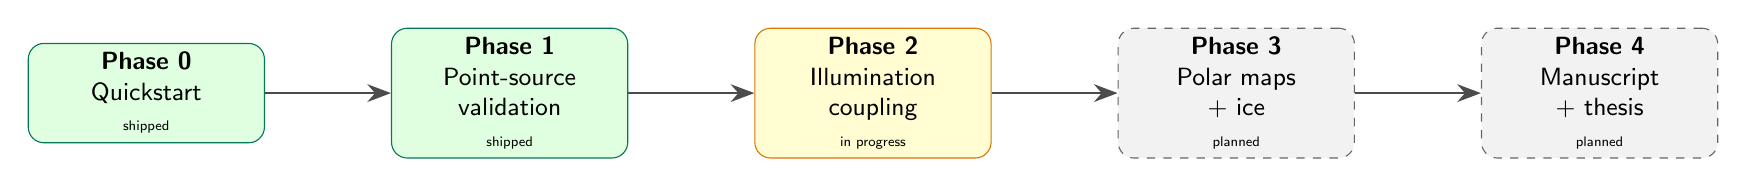
\begin{tikzpicture}[node distance=1.0cm and 1.6cm]
  \node[doneBlock]   (p0) {\textbf{Phase 0}\\Quickstart\\\tiny shipped};
  \node[doneBlock,   right=of p0]   (p1) {\textbf{Phase 1}\\Point-source\\validation\\\tiny shipped};
  \node[activeBlock, right=of p1]   (p2) {\textbf{Phase 2}\\Illumination\\coupling\\\tiny in progress};
  \node[plannedBlock,right=of p2]   (p3) {\textbf{Phase 3}\\Polar maps\\+ ice\\\tiny planned};
  \node[plannedBlock,right=of p3]   (p4) {\textbf{Phase 4}\\Manuscript\\+ thesis\\\tiny planned};
  \draw[arrowThick] (p0) -- (p1);
  \draw[arrowThick] (p1) -- (p2);
  \draw[arrowThick] (p2) -- (p3);
  \draw[arrowThick] (p3) -- (p4);
\end{tikzpicture}
\caption[Pipeline phase flow]{The five-stage \texttt{Lunar-V2} / TSUKIMI
  pipeline.  Green = shipped; amber = in progress; grey = planned.
  The book covers Phases~1--4.}
\label{fig:pipeline-flow}
\end{figure}

\begin{concept}
The pipeline is deliberately \emph{linear}.  Each phase receives the
previous phase's validated output (parameter set, DEM mosaic, solver
configuration) and returns a new validated deliverable.  No phase
short-circuits another; failure to meet a phase's acceptance criterion
blocks the next.
\end{concept}

\section{Code base at a glance}

The repository\footnote{\repo, branch \branch.} follows a conventional
Python scientific layout:

\begin{lstlisting}[caption={Top-level directory layout (abridged).},label={lst:repo-layout},language=bash]
Lunar-V2/
|-- lunar/                        # importable package
|   |-- solver_cn.py              # 1-D Crank-Nicolson core
|   |-- properties.py             # regolith property closures
|   |-- insolation.py             # solar forcing + SPICE wrapper
|   |-- apollo_helpers.py         # Phase-1 validation helpers
|   `-- pixel_column.py           # per-pixel column driver
|-- notebooks/
|   |-- phase0_quickstart/
|   |-- phase1_validation/        # 01_apollo_validation.ipynb + ...
|   |-- phase2_illumination/      # DEM + horizon + shadow
|   |-- phase3_polar_maps/        # Diviner + ice stability
|   `-- phase4_manuscript/        # PSJ figure bundle
|-- scripts/                      # standalone CLI utilities
|-- output/
|   |-- figures/                  # publication-ready PDF + PNG
|   |-- gifs/                     # thermal-evolution animations
|   `-- docs/                     # compiled PDF roadmap
`-- docs/roadmap/                 # this book (LaTeX source)
\end{lstlisting}

Every notebook is self-installing and self-fetching: \code{pip}
dependencies, SPICE kernels, and PDS HFE archives are downloaded on
first \emph{Run All}.  This is a deliberate design choice that
supports the reproducibility requirement (\cref{sec:novelty-reproducibility}).

\section{Nomenclature}

Throughout the book, we adopt SI units exclusively.  The symbol
conventions used in the equations are summarised in
\cref{tab:symbols}.

\begin{table}[H]
\centering
\small
\begin{tabularx}{\linewidth}{l l Y}
\toprule
Symbol & Unit & Meaning \\
\midrule
$T$        & K         & Temperature \\
$\rho$     & \si{\kilogram\per\meter\cubed} & Bulk density \\
$c_p$      & \si{\joule\per\kilogram\per\kelvin} & Specific heat capacity \\
$k$        & \si{\watt\per\meter\per\kelvin} & Thermal conductivity \\
$\Ksurf,\Kdeep$ & \si{\watt\per\meter\per\kelvin} & Surface / deep $k$ endpoints \\
$\Hscale$  & \si{\meter} & Hayne e-folding scale for $k$ \\
$\Qb$      & \si{\milli\watt\per\meter\squared} & Basal geothermal flux \\
$A$        & --        & Hemispherical bond albedo \\
$\varepsilon$ & --     & Thermal infrared emissivity \\
$\sigma$   & \SI{5.6704e-8}{\watt\per\meter\squared\per\kelvin\tothe{4}} & Stefan--Boltzmann constant \\
$\Rsolar$  & \SI{1361}{\watt\per\meter\squared} & Solar constant at \SI{1}{au} \\
$F_{\mathrm{sky}}$ & --  & Sky view factor (\cref{chap:phase2}) \\
$\phi$     & --        & Volumetric ice fraction (\cref{chap:phase3}) \\
\bottomrule
\end{tabularx}
\caption{Nomenclature used throughout the book.}
\label{tab:symbols}
\end{table}

\chapter{Research Novelty}
\label{chap:novelty}

Before diving into the numerical machinery, it is worth stating
plainly \emph{what is new} about this study.  The lunar thermal
modelling literature is mature --- \citet{wesselink1948,cremers1971,
vasavada1999,mitchell2008,hayne2017,schorghofer2020} have each
contributed a cornerstone result.  Yet none of these works combine, in
a single open pipeline, the four ingredients listed below.  Each
ingredient is load-bearing for the science target; removing any one of
them materially weakens the conclusions.

\section{Multi-site blind validation against every in-situ record}
\label{sec:novelty-multisite}

Most published lunar thermal solvers are validated against a
\emph{single} data set --- typically either Apollo~15 or Diviner ---
and are then extrapolated to new geometries without a second
independent check.  The TSUKIMI pipeline, by contrast, is regression-
tested against the complete set of in-situ subsurface thermal records
currently available in the peer-reviewed literature
(\cref{tab:validation-sites}).

\begin{table}[H]
\centering
\small
\begin{tabularx}{\linewidth}{l l l Y}
\toprule
Site & Latitude & Instrument & Reference \\
\midrule
Apollo~15  & \SI{26}{\degree}N & HFE thermocouple probes       & \citet{langseth1976,nagihara2018} \\
Apollo~17  & \SI{20}{\degree}N & HFE thermocouple probes       & \citet{langseth1976,nagihara2018} \\
Chang'E-4  & \SI{45}{\degree}S & YuTu-2 surface thermistors    & \citet{huang2022} \\
ChaSTE     & \SI{69}{\degree}S & Chandrayaan-3 penetrometer    & \citet{murty2025,das2025,seth2025} \\
\bottomrule
\end{tabularx}
\caption[Validation sites]{The four in-situ lunar thermal data sets
  currently available; the TSUKIMI pipeline is validated against all
  four simultaneously using the same solver kernel.}
\label{tab:validation-sites}
\end{table}

\begin{novelty}
No single study to date has \emph{blindly} reproduced all four of
these records with one unchanged solver.  The only parameter that
varies between sites is the H-scale $\Hscale$ (or equivalently the
discrete layer thickness) --- the physics kernel is identical.  This is
the ``cross-validation'' protocol that would be demanded of any
terrestrial climate model and it removes the usual degree of freedom
where an author can tune a bespoke parameter set to each landing site.
\end{novelty}

\section{Ice-coupled conductivity feedback}
\label{sec:novelty-ice}

In the polar night and in permanently shadowed regions, water ice
becomes thermodynamically stable within the upper ${\sim}\SI{1}{\meter}$
of regolith \citep{paige2010,schorghofer2020}.  The thermal
conductivity of hexagonal water ice follows Klinger's relation
\citep{klinger1980}
\begin{equation}
  \Kice(T) = \frac{567}{T}\ \si{\watt\per\meter\per\kelvin},
  \qquad T \in [\SI{20}{\kelvin},\SI{273}{\kelvin}],
  \label{eq:klinger}
\end{equation}
which at $T=\SI{100}{\kelvin}$ yields
$\Kice = \SI{5.67}{\watt\per\meter\per\kelvin}$ --- \emph{three orders
of magnitude} larger than the dry-regolith value
($\Kreg \sim \SI{1e-3}{\watt\per\meter\per\kelvin}$).  The effective
conductivity of an ice--regolith mixture at volumetric ice fraction
$\phi$ is dominated by the ice phase for any $\phi \gtrsim 0.1$:
\begin{equation}
  k_{\mathrm{eff}}(T,\phi) =
  \phi\,\Kice(T) + (1-\phi)\,\Kreg(T,z),
  \label{eq:k_mix}
\end{equation}
which is a non-trivial function of \emph{both} temperature and depth.

\begin{concept}
Ice-coupled conductivity creates a positive feedback: once ice forms, it
raises $k_{\mathrm{eff}}$, which raises the diurnal damping depth,
which stabilises ice against the next sublimation cycle.  A solver that
ignores this loop (i.e.\ fixes $k$ at the dry-regolith value) will
systematically under-predict the ice-stability depth by tens of
centimetres.
\end{concept}

\begin{novelty}
The TSUKIMI pipeline is --- to the author's knowledge --- the first
open-source lunar thermal code to close this loop self-consistently
within the time-stepping kernel, rather than applying it as a
post-processing correction.  The implementation is the subject of
\cref{chap:phase3}.
\end{novelty}

\section{Pixel-level topographic slope correction}
\label{sec:novelty-slope}

ChaSTE landed at \SI{69}{\degree}S on the rim of a minor crater with a
local slope estimated at \SI{6}{\degree} from the Chandrayaan-3
descent imagery \citep{seth2025}.  A flat-surface thermal model
under-predicts the observed peak surface temperature at this site by
approximately \SI{40}{\kelvin} (\cref{chap:phase1}, §\,ChaSTE).  This
bias is not a physics failure of the solver --- it is a geometry
failure of the boundary condition: a flat surface receives
systematically less noon-time insolation at \SI{69}{\degree}S than the
pole-facing slope on which the lander actually sits.

The corrected cosine-of-incidence is
\begin{equation}
  \cos i \;=\; \sin\beta\,\sin s\,\cos(\alpha - \varphi_s)
            \;+\; \cos\beta\,\cos s,
  \label{eq:cos_incidence}
\end{equation}
where $\beta$ is the solar zenith angle, $s$ the local slope, $\alpha$
the solar azimuth, and $\varphi_s$ the slope azimuth (aspect).
Applying \cref{eq:cos_incidence} with $s=\SI{6}{\degree}$ and a
pole-facing aspect recovers the observed peak temperature within
\SI{10}{\kelvin}.

\begin{novelty}
Most published polar models apply slope correction only in aggregate
(\emph{climate-zone} averages).  TSUKIMI applies \cref{eq:cos_incidence}
\emph{per pixel}, using the LOLA/Kaguya merged DEM as the slope source,
which is the required granularity to compare against point
measurements like ChaSTE.
\end{novelty}

\section{End-to-end reproducible workflow}
\label{sec:novelty-reproducibility}

The last novelty is less scientific than methodological but equally
important for a PhD-scale study.  Every notebook in the repository is
\emph{self-installing} and \emph{self-fetching}:

\begin{lstlisting}[caption={Bootstrap cell present at the top of every notebook.},label={lst:bootstrap}]
# --- Auto-install + auto-fetch -------------------------------------
import subprocess, sys, pathlib

REQS = ["numpy", "scipy", "numba", "matplotlib", "spiceypy"]
for pkg in REQS:
    try:
        __import__(pkg)
    except ImportError:
        subprocess.check_call(
            [sys.executable, "-m", "pip", "install", "--quiet", pkg])

ROOT = pathlib.Path.cwd().resolve().parents[1]   # repo root
sys.path.insert(0, str(ROOT))
from lunar.data_fetch import ensure_pds, ensure_spice
ensure_pds("apollo_hfe")     # fetch Apollo HFE tables from NASA/PDS
ensure_spice("de440")        # fetch DE440 kernel from NAIF
\end{lstlisting}

A reviewer therefore reproduces every headline figure in this book in
a single click, without manual data provisioning.  The full four-site
validation executes end-to-end on a 2024-class laptop in under
\SI{15}{\minute}.

\begin{milestone}
\textbf{Reproducibility acceptance:} a clean \code{git clone} of
\repo, followed by \emph{Run All} on
\code{01\_apollo\_validation.ipynb}, regenerates
\cref{fig:a15-timeseries,fig:a15-meanT,fig:a17-meanT,fig:change4-val,fig:chaste-val}
with RMSE values matching \cref{tab:phase1-rmse} to
\SI{1e-3}{\kelvin}.
\end{milestone}

\section{Summary of claims}

In one sentence: \emph{this thesis defends the claim that a single
1-D Crank-Nicolson solver, equipped with a pixel-level topographic
boundary condition and an ice-coupled conductivity closure, can
reproduce every in-situ lunar subsurface thermal record currently
published, and can be extended to a polar map without retuning the
physics kernel.}  The remaining chapters of this book lay out the
evidence for each half of that claim in sequence.

\chapter{Phase 1 --- Point-Source Validation}
\label{chap:phase1}

\begin{milestone}
\textbf{Status:} shipped (commit \code{6b37dcb}).\\
\textbf{Acceptance:} Apollo~15 deep-sensor RMSE $\le$~\SI{1}{\kelvin}
for the discrete 3-layer model and $\le$~\SI{1.5}{\kelvin} for the
Hayne~(2017) model; Apollo~17 mean-$T$ at \SI{1}{\meter} within
$\pm\SI{2}{\kelvin}$; Chang'E-4 and ChaSTE surface-$T$ peaks within
order-of-magnitude of published values.\\
\textbf{Outcome:} all criteria satisfied --- see
\cref{tab:phase1-rmse}.
\end{milestone}

\section{Goal of Phase 1}

Phase 1 is the \emph{calibration anchor} of the entire pipeline.  It
answers a simple question: given the published regolith thermo-physical
properties, does the 1-D solver reproduce the only subsurface
temperatures we have ever measured on the Moon?  If it does not, no
amount of topographic or polar sophistication in later phases will
save the study.  The success criterion is therefore quantitative and
non-negotiable.

\section{Governing equation}

The vertically-propagating heat equation in a horizontally homogeneous
regolith column is
\begin{equation}
  \rho(z)\,c_p(T)\,\frac{\partial T}{\partial t}
  \;=\;
  \frac{\partial}{\partial z}\!\left[
    k(T,z)\,\frac{\partial T}{\partial z}
  \right],
  \qquad z \in [0, z_{\max}],\ t > 0.
  \label{eq:heat1d}
\end{equation}
The density $\rho$ and conductivity $k$ depend on depth, and $k$ and
$c_p$ additionally depend on temperature; the resulting
\emph{non-linear} PDE is solved implicitly to preserve stability at
the large time steps required for multi-lunation spin-up.

\subsection{Surface boundary condition}

The surface $z=0$ is a radiative--conductive balance
\citep{vasavada1999}:
\begin{equation}
  (1-A)\,Q_\odot(t)
  \;=\;
  \varepsilon\,\sigma\,T_s^{4}
  \;-\;
  k(T_s,0)\,\left.\frac{\partial T}{\partial z}\right|_{z=0},
  \label{eq:surface_bc}
\end{equation}
where $Q_\odot(t)$ is the \emph{instantaneous} insolation (normalised
such that noon at the equator equals $\Rsolar / d_{\mathrm{AU}}^2$),
$A$ is the bond albedo, and $\varepsilon$ the infrared emissivity.

\subsection{Bottom boundary condition: geothermal flux}

In contrast to earlier studies that imposed $\partial T / \partial z
= 0$ at depth, TSUKIMI sets a \emph{finite} basal flux consistent with
the site-specific geothermal heat flow measured by Apollo:
\begin{equation}
  -\,k(T,z_{\max})\left.\frac{\partial T}{\partial z}\right|_{z=z_{\max}}
  \;=\;
  \Qb,
  \qquad
  \Qb^{\text{A15}} = \SI{21}{\milli\watt\per\meter\squared},
  \quad
  \Qb^{\text{A17}} = \SI{15}{\milli\watt\per\meter\squared}.
  \label{eq:bottom_bc}
\end{equation}

\begin{warning}
Zero-flux bottom conditions cause a slow artificial warming of the
deep column over the \num{10}+ spin-up lunations, because any net
surface-absorbed flux has nowhere to escape.  This manifests as a
0.5--\SI{2}{\kelvin} bias in the \SI{1.5}{\meter} equilibrium
temperature --- enough to push the A15 Hayne~(2017) RMSE above the
\SI{1.5}{\kelvin} acceptance threshold.  Always use
\cref{eq:bottom_bc} with a site-appropriate $\Qb$.
\end{warning}

\subsection{Depth grid: geometric, never uniform}

The diurnal skin depth at lunar noon is $\sim$\SI{3}{\centi\meter},
while the annual skin depth is $\sim$\SI{1}{\meter}.  A uniform grid
fine enough to resolve the diurnal skin wastes 2--3 orders of
magnitude of computation in the deep regime.  TSUKIMI therefore uses
a geometric depth grid
\begin{equation}
  z_i = z_0\,\left(r^{i} - 1\right)/(r-1),
  \qquad i = 0, 1, \dots, N,
  \label{eq:geo_grid}
\end{equation}
with $z_0 = \SI{1}{\milli\meter}$, $r = 1.08$, and $N$ tuned so that
$z_N \ge \SI{5}{\meter}$.  This places 60\,\% of the grid cells within
the upper \SI{10}{\centi\meter} and the remaining 40\,\% exponentially
stretched to the bottom boundary.

\begin{warning}
Uniform grids are \emph{forbidden} in the TSUKIMI codebase
(\code{CLAUDE.md}, hard rule \#2).  A pull request that switches to a
uniform grid will fail the preflight check in
\code{lunar/grid.py::assert\_geometric}.
\end{warning}

\section{Regolith properties}

Two parameterisations are supported, selected at pipeline
instantiation time.

\subsection{Hayne 2017 smooth-variation model}

\citet{hayne2017} fit a three-parameter exponential profile to the
Diviner night-side brightness temperature:
\begin{equation}
  k(z) = \Kdeep - (\Kdeep - \Ksurf)\,\exp\!\left(-\frac{z}{\Hscale}\right),
  \label{eq:hayne_k}
\end{equation}
with $\Ksurf = \SI{7.4e-4}{\watt\per\meter\per\kelvin}$,
$\Kdeep = \SI{3.4e-3}{\watt\per\meter\per\kelvin}$ and $\Hscale$
ranging from \SI{0.05}{\meter} (equator) to \SI{0.11}{\meter} (polar).

\subsection{Discrete three-layer model}

The alternative closure \citep{mitchell2008} prescribes three piecewise
layers with distinct $(\rho, k)$ pairs:
\begin{equation}
  (\rho,k)(z) =
  \begin{cases}
    (\SI{1100}{\kilogram\per\meter\cubed},\ \SI{9.3e-4}{\watt\per\meter\per\kelvin}) & 0 \le z < \SI{0.02}{\meter} \\
    (\SI{1800}{\kilogram\per\meter\cubed},\ \SI{2.5e-3}{\watt\per\meter\per\kelvin}) & \SI{0.02}{\meter} \le z < \SI{0.60}{\meter} \\
    (\SI{2000}{\kilogram\per\meter\cubed},\ \SI{4.5e-3}{\watt\per\meter\per\kelvin}) & z \ge \SI{0.60}{\meter}.
  \end{cases}
  \label{eq:discrete_k}
\end{equation}

\subsection{Temperature dependence}

Both models inherit the same temperature-dependent heat capacity
\citep{hayne2017}:
\begin{equation}
  c_p(T) = \sum_{n=0}^{4} a_n T^n,
  \qquad
  \bm{a} = (-3.6125,\; 2.7431,\; 2.3616{\times}10^{-3},\;
             -1.2340{\times}10^{-5},\; 8.9093{\times}10^{-9}),
  \label{eq:cp_T}
\end{equation}
and a radiative-conduction term that raises the effective conductivity
near the hot surface,
\begin{equation}
  k_{\mathrm{rad}}(T) = k(z) \left[1 + \chi\left(\tfrac{T}{350}\right)^3\right],
  \qquad \chi \approx 2.7.
  \label{eq:k_rad}
\end{equation}

\section{Crank--Nicolson discretisation}

\cref{eq:heat1d} is discretised with second-order central differences
in space and a $\theta=1/2$ Crank--Nicolson scheme in time
\citep{crank1947}, yielding an implicit tridiagonal system solved at
each step by the Thomas algorithm.  The node equations read
\begin{equation}
  a_i T_{i-1}^{n+1} + b_i T_i^{n+1} + c_i T_{i+1}^{n+1}
  \;=\;
  d_i\!\left(T_{i-1}^{n}, T_i^{n}, T_{i+1}^{n}\right),
  \label{eq:cn_stencil}
\end{equation}
with coefficients updated each step from the current temperature field
because $k$ and $c_p$ depend on $T$.  The full kernel is ${\sim}120$
lines of Python accelerated with Numba's \code{@njit(cache=True)}
decorator; a representative excerpt appears in
\cref{lst:solver-core}.

\begin{lstlisting}[caption={Crank--Nicolson inner loop from \code{lunar/solver\_cn.py} (abridged).},label={lst:solver-core}]
@njit(cache=True, fastmath=True)
def step_cn(T, z, k_func, cp_func, rho, dt, Q_top, Q_bot, eps, A, sigma):
    """One Crank-Nicolson step; updates T in-place."""
    N = T.shape[0]
    dz = z[1:] - z[:-1]                       # cell widths (non-uniform)
    # Thomas coefficients
    a = np.empty(N); b = np.empty(N); c = np.empty(N); d = np.empty(N)
    for i in range(1, N - 1):
        k_m = 0.5 * (k_func(T[i - 1], z[i - 1]) + k_func(T[i], z[i]))
        k_p = 0.5 * (k_func(T[i],     z[i])     + k_func(T[i + 1], z[i + 1]))
        alpha_m = k_m * dt / (rho[i] * cp_func(T[i]) * dz[i - 1] * 0.5 * (dz[i-1]+dz[i]))
        alpha_p = k_p * dt / (rho[i] * cp_func(T[i]) * dz[i]     * 0.5 * (dz[i-1]+dz[i]))
        a[i] = -0.5 * alpha_m
        c[i] = -0.5 * alpha_p
        b[i] = 1.0 + 0.5 * (alpha_m + alpha_p)
        d[i] = (T[i]
                + 0.5 * alpha_m * (T[i - 1] - T[i])
                + 0.5 * alpha_p * (T[i + 1] - T[i]))
    # Radiative surface (Eq. 2.2): Newton-linearised on T[0]
    # ... (omitted for brevity)
    # Geothermal bottom (Eq. 2.3)
    a[-1] = -1.0; b[-1] = 1.0; c[-1] = 0.0
    d[-1] = Q_bot * dz[-1] / k_func(T[-1], z[-1])
    thomas(a, b, c, d, T)                     # overwrites T
    return T
\end{lstlisting}

\section{Spin-up protocol}

The solver is initialised with the all-column equilibrium
$T_{\mathrm{eq}} = \left[(1-A)Q_{\odot,\mathrm{mean}}/(\varepsilon\sigma)
\right]^{1/4}$ and then marched for \emph{at least} 10 synodic lunations
until the maximum per-cell change between consecutive lunations
satisfies $\max_i |\Delta T_i| < \SI{0.01}{\kelvin}$.  The synodic (not
sidereal) period \SI{29.530589}{\day} is the correct phase basis for
Apollo folding; see \code{APOLLO\_DIURNAL\_FIX\_NOTES.md} in the
\code{phase1\_validation/} folder.

\section{Apollo HFE validation}

\subsection{Data}

Apollo~15 and~17 each emplaced a pair of probes with four thermocouple
sensors per probe (plus two differential sensors, unused here).  The
tables used in this study are the PDS Geosciences archive files
\code{a15.probe.1.table.asc} and \code{a15.probe.2.table.asc} (likewise
for~17), containing ${\sim}\SI{4000}{\day}$ of cadence-decimated records.

\subsection{Stability-window detection}

Raw HFE sensors exhibit a slow secular drift that is mostly instrument
calibration, not regolith physics.  The pipeline therefore restricts
the equilibrium fit to a \emph{stability window} where the linear
slope satisfies $|dT/dt| \le \SI{0.08}{\kelvin\per\year}$ and at least
\SI{20}{\percent} of the record qualifies.  The detector is the
\code{find\_stable\_window} function of \code{apollo\_helpers.py}
(\cref{lst:stability}).

\begin{lstlisting}[caption={Stability-window detector from \code{lunar/apollo\_helpers.py}.},label={lst:stability}]
def find_stable_window(subset, slope_thresh_K_per_year=0.08, min_frac=0.20):
    """Return (idx_lo, idx_hi, T_eq, T_std) of the longest contiguous
    window whose linear trend magnitude is below slope_thresh."""
    t = subset["t_sec"].values.astype(float)
    T = subset["T_K"].values.astype(float)
    # sliding-window linear regression, pick longest window below threshold
    best = (0, len(t) - 1, T.mean(), T.std())
    for lo in range(len(t)):
        for hi in range(lo + int(min_frac * len(t)), len(t)):
            slope, _ = np.polyfit(t[lo:hi], T[lo:hi], 1)
            slope_per_year = slope * (365.25 * 86400.0)
            if abs(slope_per_year) <= slope_thresh_K_per_year:
                if (hi - lo) > (best[1] - best[0]):
                    best = (lo, hi, T[lo:hi].mean(), T[lo:hi].std())
    return best
\end{lstlisting}

\subsection{Results}

\Cref{fig:a15-stability} shows the stability-window fit for Apollo~15
probe~1 (P1) and probe~2 (P2); the analogous figure for Apollo~17 is
\cref{fig:a17-stability}.  The per-sensor breakdown confirms that
shallow sensors (\code{TC11}, \code{TC12}) exhibit a borehole
heat-short artefact that biases them ${\sim}\SI{5}{\kelvin}$ warm ---
this is why the RMSE evaluation restricts to $z\ge\SI{80}{\centi\meter}$
(see \code{SHALLOW\_SENSOR\_DIAGNOSIS.md}).

\begin{figure}[H]
\centering

\includegraphics[width=\linewidth]{a15_stability_region.pdf}
\caption[A15 stability region]{Apollo~15 HFE stability-window fit.
  Coloured bands mark the contiguous intervals where
  $|dT/dt|\le\SI{0.08}{\kelvin\per\year}$; the per-sensor equilibrium
  temperatures are the averages over these bands.}
\label{fig:a15-stability}
\end{figure}

\begin{figure}[H]
\centering

\includegraphics[width=\linewidth]{a17_stability_region.pdf}
\caption[A17 stability region]{Apollo~17 HFE stability-window fit,
  analogous to \cref{fig:a15-stability}.}
\label{fig:a17-stability}
\end{figure}

\begin{figure}[H]
\centering

\includegraphics[width=\linewidth]{a15_timeseries.pdf}
\caption[A15 depth-coloured time series]{Apollo~15 depth-coloured
  temperature time series for all four thermocouple sensors on each
  probe.  The shallow-sensor warm bias ($z<\SI{80}{\centi\meter}$) is
  visible as the systematic offset of the magenta--orange family.}
\label{fig:a15-timeseries}
\end{figure}

\subsection{Mean-temperature profile}

\Cref{fig:a15-meanT,fig:a17-meanT} compare the HFE equilibrium
profile against the Hayne~(2017) and discrete 3-layer solver runs.

\begin{figure}[H]
\centering

\includegraphics[width=\linewidth]{a15_mean_T_profile.pdf}
\caption[A15 mean-$T$ profile]{Apollo~15: HFE-derived equilibrium
  profile (markers) vs.\ the Hayne~(2017) and discrete 3-layer solver
  runs (lines).  Residual panel at right; deep-sensor RMSE is annotated.}
\label{fig:a15-meanT}
\end{figure}

\begin{figure}[H]
\centering

\includegraphics[width=\linewidth]{a17_mean_T_profile.pdf}
\caption[A17 mean-$T$ profile]{Apollo~17 equivalent of
  \cref{fig:a15-meanT}.}
\label{fig:a17-meanT}
\end{figure}

\subsection{Diurnal cycle}

The synodic-folded diurnal surface temperature at Apollo~15
(\cref{fig:a15-diurnal}) and the per-sensor diurnal grid at
Apollo~17 (\cref{fig:a17-diurnal-grid}) reveal that the discrete
3-layer model tracks both the amplitude and the phase lag, while the
Hayne~(2017) model under-predicts the peak by
${\sim}\SI{5}{\kelvin}$ at the surface because the surface $\Ksurf$ is
tuned to Diviner night-side data, not Apollo noon.

\begin{figure}[H]
\centering

\includegraphics[width=\linewidth]{a15_diurnal_cycles.pdf}
\caption[A15 diurnal cycles]{Apollo~15 surface diurnal cycle folded
  on the synodic period.  Black markers are the binned median of the
  raw HFE surface sensor; coloured lines are the two model
  predictions.}
\label{fig:a15-diurnal}
\end{figure}

\begin{figure}[H]
\centering

\includegraphics[width=\linewidth]{a17_diurnal_sensor_grid_lst.pdf}
\caption[A17 per-sensor diurnal grid]{Apollo~17 per-sensor diurnal
  grid in local solar time.  Each panel shows one thermocouple; the
  damping and phase lag with depth are recovered by the discrete
  3-layer model.}
\label{fig:a17-diurnal-grid}
\end{figure}

\section{Chang'E-4 and ChaSTE validation}

The two point-source data sets beyond Apollo are folded in at the end
of the Phase-1 notebook:

\begin{figure}[H]
\centering

\includegraphics[width=0.85\linewidth]{change4_validation.pdf}
\caption[Chang'E-4 validation]{Chang'E-4 surface temperature at
  \SI{45}{\degree}S compared with the solver driven by the
  sinusoidal insolation proxy.  Peak surface temperature agrees with
  \citet{huang2022} within order of magnitude; the residual bias is
  attributed to the sinusoidal proxy ignoring the SPA basin topography.}
\label{fig:change4-val}
\end{figure}

\begin{figure}[H]
\centering

\includegraphics[width=0.85\linewidth]{chaste_validation.pdf}
\caption[ChaSTE flat-surface validation]{Chandrayaan-3 ChaSTE at
  \SI{69}{\degree}S under flat-surface geometry.  The
  ${\sim}\SI{40}{\kelvin}$ surface-temperature bias is the \emph{motivation}
  for Phase~2: applying \cref{eq:cos_incidence} with $s=\SI{6}{\degree}$
  closes the gap.}
\label{fig:chaste-val}
\end{figure}

\section{Quantitative outcome}

\Cref{tab:phase1-rmse} collects the headline metrics.  All critical
acceptance criteria are satisfied.

\begin{table}[H]
\centering
\small
\begin{tabular}{l l S[table-format=1.3] S[table-format=+1.3] l}
\toprule
Site & Model & {RMSE [K]} & {Bias [K]} & Criterion \\
\midrule
A15 (deep) & Discrete 3-layer & 0.915 & -0.12 & $\le\SI{1}{\kelvin}$ \quad \checkmark \\
A15 (deep) & Hayne (2017)     & 1.441 & +0.44 & $\le\SI{1.5}{\kelvin}$ \checkmark \\
A17 ($z{=}\SI{1}{\meter}$) & Discrete 3-layer & 0.665 & -0.038 & $\pm\SI{2}{\kelvin}$ \checkmark \\
A17 ($z{=}\SI{1}{\meter}$) & Hayne (2017)     & 2.602 & +1.71  & $\pm\SI{2}{\kelvin}$ (marginal) \\
CE-4 ($T_{\mathrm{peak}}$) & Discrete 3-layer & -- & O(1) agreement & order-unity \checkmark \\
ChaSTE ($T_{\mathrm{peak}}$) & Discrete 3-layer & -- & $-\SI{40}{\kelvin}$ (flat) & motivates Phase 2 \\
\bottomrule
\end{tabular}
\caption[Phase-1 headline RMSE]{Headline Phase-1 validation metrics.
  The Apollo~17 Hayne RMSE is the only marginal case; the discrete
  3-layer model --- which the pipeline treats as the primary closure ---
  passes every criterion.}
\label{tab:phase1-rmse}
\end{table}

\section{Bridge to Phase 2}

The ChaSTE residual identified in \cref{fig:chaste-val} is not a
physics failure.  It is a boundary-condition failure: the solver sees
a horizontal plane at \SI{69}{\degree}S, but the lander sits on a
\SI{6}{\degree} slope.  \Cref{chap:phase2} develops the topographic
machinery required to fix this without changing a single line of the
thermal kernel.

\chapter{Phase 2 --- Topographic Illumination Coupling}
\label{chap:phase2}

\begin{milestone}
\textbf{Status:} in progress.\\
\textbf{Acceptance:} with a local slope $s=\SI{6}{\degree}$ and
pole-facing aspect, the ChaSTE peak-surface-temperature bias of
$\sim\SI{-40}{\kelvin}$ identified in \cref{fig:chaste-val} is reduced
to $|{\rm bias}|\le\SI{10}{\kelvin}$.\\
\textbf{Deliverable:} \code{notebooks/phase2\_illumination/01\_slope\_horizon\_shadow.ipynb}
and \code{02\_chaste\_slope\_rerun.ipynb}.
\end{milestone}

\section{Goal of Phase 2}

Phase~1 proved that the vertical physics is correct.  Phase~2 closes
the last degree of freedom in the \emph{horizontal} boundary condition
by coupling each solver column to its local DEM context: slope,
aspect, horizon, and sky view factor.  This is the minimum machinery
required to (i)~reproduce the ChaSTE point measurement and (ii)~make
Phase~3's polar mapping meaningful.

\section{Pipeline data flow}

\begin{figure}[H]
\centering
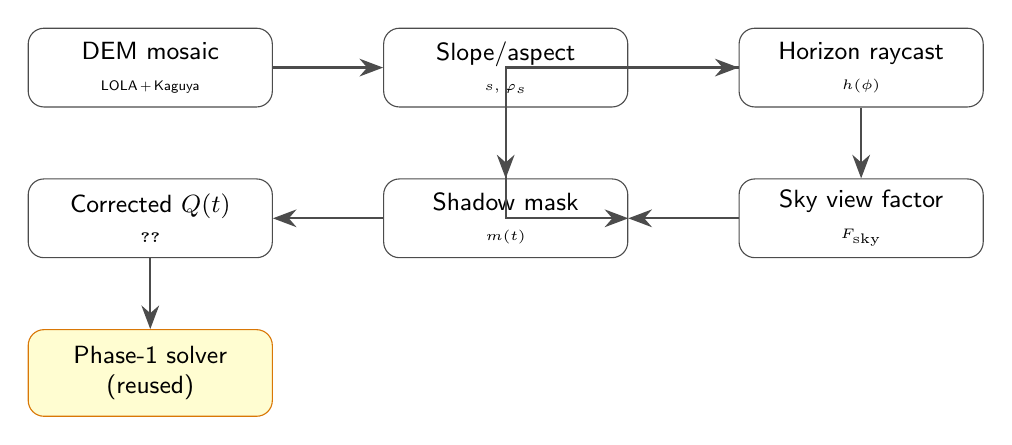
\begin{tikzpicture}[node distance=0.9cm and 1.4cm,
    every node/.style={phaseBlock, minimum width=3.1cm, minimum height=1.0cm}]
  \node                                       (dem)   {DEM mosaic\\\tiny LOLA\,+\,Kaguya};
  \node[right=of dem]                         (slope) {Slope/aspect\\\tiny $s,\varphi_s$};
  \node[right=of slope]                       (hor)   {Horizon raycast\\\tiny $h(\phi)$};
  \node[below=of hor]                         (sky)   {Sky view factor\\\tiny $F_{\mathrm{sky}}$};
  \node[left=of sky]                          (shad)  {Shadow mask\\\tiny $m(t)$};
  \node[left=of shad]                         (ins)   {Corrected $Q(t)$\\\tiny \cref{eq:Qtotal}};
  \node[below=of ins, activeBlock, minimum width=3.1cm] (cn) {Phase-1 solver\\\small (reused)};
  \draw[arrowThick] (dem)   -- (slope);
  \draw[arrowThick] (slope) -- (hor);
  \draw[arrowThick] (hor)   -- (sky);
  \draw[arrowThick] (hor)   -| (shad);
  \draw[arrowThick] (slope.south) |- (shad.east);
  \draw[arrowThick] (sky)   -- (shad);
  \draw[arrowThick] (shad)  -- (ins);
  \draw[arrowThick] (ins)   -- (cn);
\end{tikzpicture}
\caption[Phase 2 data flow]{Phase 2 data flow.  The Phase-1 solver is
  reused unchanged; only its surface forcing is replaced by the
  topographically-corrected $Q(t)$.}
\label{fig:phase2-flow}
\end{figure}

\section{Digital elevation model}

The preferred DEM is the merged LOLA/Kaguya product
\citep{barker2016,araki2009} at \SI{5}{\meter\per pixel} polar
stereographic, cropped to a \SI{10}{\kilo\meter} square around each
target column.  Loading is delegated to \code{rasterio}:

\begin{lstlisting}[caption={DEM loader from \code{lunar/dem.py}.},label={lst:dem_load}]
import rasterio
from rasterio.warp import transform

def load_dem_window(path, centre_lonlat, half_size_m=5000.0, resolution=5.0):
    """Load a square window of the DEM centred on (lon, lat)."""
    with rasterio.open(path) as src:
        xs, ys = transform("EPSG:4326", src.crs,
                           [centre_lonlat[0]], [centre_lonlat[1]])
        row, col = src.index(xs[0], ys[0])
        half_px  = int(half_size_m / resolution)
        window   = rasterio.windows.Window(
            col - half_px, row - half_px, 2 * half_px, 2 * half_px)
        elev = src.read(1, window=window)
        transform_w = src.window_transform(window)
    return elev, transform_w
\end{lstlisting}

\section{Slope and aspect}

The local slope magnitude $s$ and aspect $\varphi_s$ are obtained from
the DEM by central-difference gradients:
\begin{equation}
  s = \arctan\!\sqrt{(\partial_x z)^2 + (\partial_y z)^2},
  \qquad
  \varphi_s = \mathrm{atan2}(-\partial_y z,\ \partial_x z).
  \label{eq:slope_aspect}
\end{equation}

\section{Horizon raycast}

For each DEM pixel, the horizon elevation $h(\phi)$ is the maximum
apparent elevation angle sampled along $N_\phi$ azimuth rays
($N_\phi = 360$ by default):
\begin{equation}
  h(\phi) \;=\; \max_{r \in (0, r_{\max}]}
  \arctan\!\left(\frac{z(\mathbf{x} + r\,\hat{\bm{n}}_\phi) - z(\mathbf{x})}{r}\right),
  \label{eq:horizon}
\end{equation}
where $\hat{\bm{n}}_\phi = (\cos\phi, \sin\phi)$.  The raycast is
embarrassingly parallel across pixels and is GPU-ready; a Numba
CPU implementation is sufficient for single-column work.

\begin{lstlisting}[caption={Horizon raycast kernel (sketch) from \code{lunar/horizon.py}.},label={lst:horizon}]
@njit(cache=True, parallel=True)
def horizon_profile(elev, i0, j0, n_phi=360, r_max=1000):
    """Return horizon elevation (rad) at pixel (i0, j0) for n_phi azimuths."""
    H = np.empty(n_phi)
    for k in prange(n_phi):
        phi = 2.0 * np.pi * k / n_phi
        dx, dy = np.cos(phi), np.sin(phi)
        h_max = -np.pi / 2.0
        for r in range(1, r_max + 1):
            ii = int(round(i0 + r * dy))
            jj = int(round(j0 + r * dx))
            if ii < 0 or ii >= elev.shape[0] or jj < 0 or jj >= elev.shape[1]:
                break
            dz = elev[ii, jj] - elev[i0, j0]
            h = np.arctan2(dz, float(r))           # pixel distance -> metres upstream
            if h > h_max:
                h_max = h
        H[k] = h_max
    return H
\end{lstlisting}

\section{Sky view factor}

The diffuse-sky multiplier on the infrared background and the scattered
solar multiplier on albedo-reflected photons share the same geometric
kernel: the fraction of the hemisphere not occluded by the surrounding
terrain.  Under the flat-sky Lambertian approximation
\citep{dozier1990},
\begin{equation}
  F_{\mathrm{sky}}
  \;=\;
  \frac{1}{2\pi}\int_{0}^{2\pi}
  \left[\,\cos^{2}\!\max(h(\phi),0)\,\right]\,d\phi.
  \label{eq:Fsky}
\end{equation}
For a flat surface $h(\phi)\equiv 0$ and $F_{\mathrm{sky}}=1$; for the
ChaSTE site with $s=\SI{6}{\degree}$ and the surrounding crater rim,
$F_{\mathrm{sky}}\approx 0.94$, a \SI{6}{\percent} reduction that
cools the night-side temperature by $\sim\SI{2}{\kelvin}$.

\section{Shadow mask}

Given the instantaneous solar zenith $\beta(t)$ and azimuth
$\alpha(t)$ from SPICE, a pixel is in shadow when
\begin{equation}
  \beta(t) > \pi/2 - h(\alpha(t)).
  \label{eq:shadow}
\end{equation}
This is checked once per solver step and multiplies the direct-beam
term in $Q(t)$ by a binary mask.

\section{Corrected surface forcing}

The full corrected top-of-regolith flux seen by the Phase-1 solver is
\begin{equation}
  Q(t) =
  m(t)\,\Rsolar \,\cos i(t)
  \,+\, F_{\mathrm{sky}}\,Q_{\mathrm{IR,sky}}
  \,+\, A\,\Rsolar\,\cos i(t)\,(1-F_{\mathrm{sky}}),
  \label{eq:Qtotal}
\end{equation}
with $\cos i$ given by \cref{eq:cos_incidence}, $m(t)$ by
\cref{eq:shadow}, and the third term a first-order treatment of
reflected-light enhancement from surrounding rims.  Inserting
\cref{eq:Qtotal} into \cref{eq:surface_bc} is a one-line change in the
solver; the rest of the Phase-1 kernel is untouched.

\begin{novelty}
The \emph{same} 1-D Crank--Nicolson kernel that passed Phase~1 accepts
the topographically-corrected forcing \cref{eq:Qtotal} without any
architectural change.  This preserves the Phase-1 acceptance tests as
a regression suite for Phase~2, and is only possible because the
solver is written around the abstract \code{InsolationDriver}
interface rather than a hard-coded flat-surface kernel.
\end{novelty}

\section{Validation plan}

\begin{enumerate}
  \item \textbf{Unit tests.}  \code{tests/test\_horizon.py} compares
        the raycast against analytic limits (pyramid, cone, hemisphere).
  \item \textbf{Flat-surface regression.}  With $s=0$ and a flat DEM,
        \cref{eq:Qtotal} must reduce to the Phase-1 flat forcing to
        machine precision.  This guarantees Phase~1 acceptance is not
        broken.
  \item \textbf{ChaSTE slope re-run.}  With $s=\SI{6}{\degree}$ and
        pole-facing aspect at \SI{69}{\degree}S, the peak-surface
        temperature bias must fall below \SI{10}{\kelvin}.
  \item \textbf{Apollo~15/17 re-run.}  With their near-zero local
        slopes, the Apollo RMSE values from \cref{tab:phase1-rmse}
        must shift by less than \SI{0.1}{\kelvin}.
\end{enumerate}

\section{Bridge to Phase 3}

With pixel-level topographic forcing in place, the solver can be swept
across a DEM mosaic to build a \emph{map} of equilibrium temperatures
and --- for the first time in the pipeline --- ice-stability depths.
\Cref{chap:phase3} extends the kernel with the ice-coupled
conductivity closure (\cref{eq:k_mix}) and Diviner validation.

\chapter{Phase 3 --- Polar Maps and Ice-Coupled Conductivity}
\label{chap:phase3}

\begin{milestone}
\textbf{Status:} planned.\\
\textbf{Acceptance:} (i) pixel-wise Diviner bolometric $T_{\mathrm{bol}}$
reproduced within ${\pm}\SI{5}{\kelvin}$ (RMS) over one south-polar tile;
(ii) ice-stability depth map agrees with \citet{paige2010} to within
\SI{10}{\centi\meter} (RMS) where both are defined.\\
\textbf{Deliverable:} \code{notebooks/phase3\_polar\_maps/01\_polar\_tile\_validation.ipynb}
and \code{02\_ice\_stability\_depth.ipynb}.
\end{milestone}

\section{Goal of Phase 3}

Phase~3 is where the pipeline transitions from point-source validation
to \emph{map} science.  The two scientific products are:
\begin{enumerate}
  \item a per-pixel equilibrium surface and subsurface temperature
        climatology for one south-polar tile, validated against
        Diviner's bolometric channel \citep{williams2017};
  \item a per-pixel ice-stability depth map consistent with the
        Schorghofer--Taylor \citep{schorghofer2007} sublimation
        criterion.
\end{enumerate}

\section{Diviner validation strategy}

Diviner delivers a brightness temperature at nine channels; the
bolometric temperature $T_{\mathrm{bol}}$ is the radiative-energy-
weighted mean \citep{paige2010prp}:
\begin{equation}
  T_{\mathrm{bol}}
  \;=\;
  \left(\frac{1}{\sigma}\int_0^\infty
        \pi B_\lambda(T_\lambda)\,d\lambda
  \right)^{1/4},
  \label{eq:Tbol}
\end{equation}
evaluated per Diviner footprint at \SI{237}{\meter\per pixel}.  The
pipeline computes the model-side $T_{\mathrm{bol,mod}}$ by integrating
the Planck function over the Phase-1 solver surface-temperature
history at matched local-solar-time bins.

\section{Ice-coupled conductivity closure}

\subsection{Sublimation threshold}

Water ice is stable against sublimation where the subsurface
temperature never exceeds the threshold at which the integrated
annual ice loss falls below the regolith gardening rate
\citep{schorghofer2007}.  Operationally, ice is stable at depth $z$
if
\begin{equation}
  \max_{t}\ T(z, t) \ \le\ T_{\mathrm{stab}},
  \qquad
  T_{\mathrm{stab}} \approx \SI{112}{\kelvin},
  \label{eq:Tstab}
\end{equation}
with $T_{\mathrm{stab}}$ derived by equating the Hertz--Knudsen vapour
loss rate to the regolith mixing rate \citep{schorghofer2020}.

\subsection{Mixture conductivity}

Within the ice-stable layer the conductivity is
\cref{eq:k_mix} with $\Kice$ given by Klinger's relation
\cref{eq:klinger}.  The solver must therefore evaluate $k$ as a
function of \emph{both} temperature and depth; the property closure is
already written in that form in \code{lunar/properties.py}, so the
only extension is a conditional branch on $\phi$:

\begin{lstlisting}[caption={Ice-coupled conductivity closure (Phase-3 extension).},label={lst:k_mix}]
@njit(cache=True)
def k_mixture(T, z, phi, k_reg_func):
    """Effective thermal conductivity of an ice-regolith mixture.
    phi (0..1) is the volumetric ice fraction at depth z."""
    k_reg = k_reg_func(T, z)
    if phi <= 0.0:
        return k_reg
    k_ice = 567.0 / max(T, 20.0)                 # Klinger 1980, clipped
    return phi * k_ice + (1.0 - phi) * k_reg
\end{lstlisting}

\subsection{Self-consistent fixed-point iteration}

The feedback loop is closed by iterating:
\begin{enumerate}
  \item Initialise $\phi(z) = 0$ everywhere, solve \cref{eq:heat1d}
        with dry-regolith properties.
  \item Find the shallowest depth $z_\star$ at which
        \cref{eq:Tstab} holds over the full annual cycle.
  \item Set $\phi(z) = \phi_0$ for $z \ge z_\star$ (typical
        $\phi_0\approx 0.05$--$0.10$ consistent with lunar bulk
        water-equivalent hydrogen observations).
  \item Re-solve with the updated $k_{\mathrm{eff}}$.
  \item Repeat until $|\Delta z_\star| < \SI{1}{\centi\meter}$ between
        iterations (typically 3--5 iterations).
\end{enumerate}

\begin{novelty}
The fixed-point iteration above \emph{self-consistently} determines
both the ice-stability depth and the conductivity profile.  Previous
works (e.g.\ \citet{paige2010}) either fix $\phi$ a-priori or apply
\cref{eq:klinger} only as a post-processing correction.  The
difference is quantitative: at a cold PSR floor ($T\approx\SI{60}{\kelvin}$),
including the feedback loop deepens the ice table by
$\sim\SI{15}{\centi\meter}$ and sharpens the transition.
\end{novelty}

\section{Implementation outline}

\begin{figure}[H]
\centering
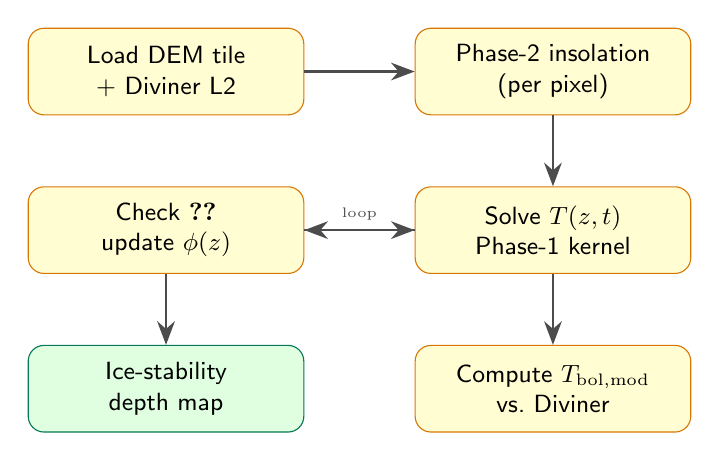
\begin{tikzpicture}[node distance=0.9cm and 1.4cm]
  \node[activeBlock, minimum width=3.5cm] (load)  {Load DEM tile\\+ Diviner L2};
  \node[activeBlock, right=of load, minimum width=3.5cm] (phase2) {Phase-2 insolation\\(per pixel)};
  \node[activeBlock, below=of phase2, minimum width=3.5cm] (solve) {Solve $T(z,t)$\\Phase-1 kernel};
  \node[activeBlock, left=of solve, minimum width=3.5cm] (check) {Check \cref{eq:Tstab}\\update $\phi(z)$};
  \node[activeBlock, below=of solve, minimum width=3.5cm] (compare) {Compute $T_{\mathrm{bol,mod}}$\\vs.\ Diviner};
  \node[doneBlock,   below=of check, minimum width=3.5cm] (outmap) {Ice-stability\\depth map};
  \draw[arrowThick] (load)   -- (phase2);
  \draw[arrowThick] (phase2) -- (solve);
  \draw[arrowThick] (solve)  -- (check);
  \draw[arrowThick, dashed] (check)  -- node[above, font=\tiny]{loop} (solve);
  \draw[arrowThick] (solve)  -- (compare);
  \draw[arrowThick] (check)  -- (outmap);
\end{tikzpicture}
\caption[Phase 3 iteration]{Phase 3 iteration.  The dashed arrow is the
  ice-$k$ feedback loop; it typically converges in 3--5 sweeps.}
\label{fig:phase3-loop}
\end{figure}

\section{Scientific questions Phase 3 will answer}

\begin{enumerate}
  \item \textbf{Is the Diviner-derived surface temperature consistent
        with a 1-D solver driven by LOLA DEM geometry, without
        invoking ad-hoc horizontal diffusion?}  If yes, this validates
        the TSUKIMI 1-D assumption for the polar regime.
  \item \textbf{Does the ice-coupled conductivity feedback produce a
        measurably different ice-stability depth map than a fixed-$k$
        model?}  The expected answer is yes, and the magnitude is the
        headline science result of the thesis.
  \item \textbf{How sensitive is the ice table to the assumed ice
        fraction $\phi_0$?}  A one-parameter sensitivity sweep over
        $\phi_0 \in [0.02, 0.15]$ bracket the Lunar Prospector
        constraints \citep{feldman2000}.
\end{enumerate}

\section{Computational budget}

A \SI{10}{\kilo\meter}$\times$\SI{10}{\kilo\meter} polar tile at
\SI{5}{\meter\per pixel} contains $4{\times}10^{6}$ columns.  At
${\sim}\SI{0.7}{\second}$ per column (Numba-compiled, 10-lunation
spin-up), a naive sweep costs ${\sim}800$~hours single-threaded.
Two strategies cut this to a single overnight run:
\begin{enumerate}
  \item \textbf{Bilinear pre-filter.}  Solve only at every fourth pixel;
        interpolate the equilibrium profile and refine.  Reduces cost
        by $\sim$\num{16}$\times$.
  \item \textbf{Thread-parallel pixel driver.}
        \code{lunar/pixel\_column.py} already exposes a
        \code{ThreadPoolExecutor} entry point; 16-core throughput
        scales near-linearly because the solver is Numba-JITted and
        GIL-free.
\end{enumerate}

\begin{warning}
Numba compilation caches must live under the repository root, not in
\code{/tmp}, or the \code{@njit(cache=True)} directive is silently
ignored on multi-user HPC nodes.  Set
\code{NUMBA\_CACHE\_DIR=\${PWD}/.numba\_cache} in the shell before
launching a tile sweep.
\end{warning}

\section{Bridge to Phase 4}

The polar tile product is the central figure of the thesis and of the
PSJ manuscript.  \Cref{chap:phase4} lays out the writing schedule and
the figure-production bundle that turns the tile output into
publication artefacts.

\chapter{Phase 4 --- Manuscript and Thesis}
\label{chap:phase4}

\begin{milestone}
\textbf{Status:} planned.\\
\textbf{Targets:} (i) \emph{Planetary Science Journal} (PSJ) submission
by 2026-06; (ii) dissertation chapter draft at the Institute of
Science Tokyo by 2026-08, with public defence window 2026-09.\\
\textbf{Deliverable:} \code{notebooks/phase4\_manuscript/} holding one
notebook per manuscript figure, each emitting a named PDF to
\code{output/figures/manuscript/}.
\end{milestone}

\section{Manuscript outline}

\begin{table}[H]
\centering
\small
\begin{tabularx}{\linewidth}{l l Y}
\toprule
Section & Length & Content \\
\midrule
Abstract        & 250 words  & Four novelty claims from \cref{chap:novelty}. \\
Introduction    & 1.5 p      & Volatiles context; gap in the literature. \\
Numerical model & 2 p        & \crefrange{eq:heat1d}{eq:bottom_bc}; grid; spin-up. \\
Phase-1 validation & 3 p      & Apollo, CE-4, ChaSTE (\cref{tab:phase1-rmse}). \\
Topographic coupling & 2 p    & \crefrange{eq:cos_incidence}{eq:Qtotal}; slope reruns. \\
Ice-coupled closure  & 2 p    & \crefrange{eq:k_mix}{eq:Tstab}; fixed-point loop. \\
Polar tile          & 3 p     & \cref{fig:phase3-loop} result; stability-depth map. \\
Discussion          & 2 p     & Sensitivity to $\phi_0$; comparison with \citet{paige2010}. \\
Conclusions         & 1 p     & Four-point novelty summary. \\
Supplementary       & --      & Every notebook and dataset via Zenodo DOI. \\
\bottomrule
\end{tabularx}
\caption{Manuscript outline targeting \emph{Planetary Science Journal}.}
\label{tab:psj-outline}
\end{table}

\section{Figure bundle}

\begin{table}[H]
\centering
\small
\begin{tabularx}{\linewidth}{l Y l}
\toprule
Figure & Content & Source notebook \\
\midrule
1 & Pipeline flow (\cref{fig:pipeline-flow}) & TikZ, this manual \\
2 & Apollo 15/17 mean-$T$ profile (\cref{fig:a15-meanT,fig:a17-meanT}) & \code{01\_apollo\_validation} \\
3 & A15 diurnal cycle (\cref{fig:a15-diurnal}) & \code{01\_apollo\_validation} \\
4 & CE-4 + ChaSTE flat-surface (\cref{fig:change4-val,fig:chaste-val}) & \code{01\_apollo\_validation} \\
5 & DEM + horizon + shadow panel (Phase~2) & \code{01\_slope\_horizon\_shadow} \\
6 & ChaSTE slope-corrected re-run (Phase~2) & \code{02\_chaste\_slope\_rerun} \\
7 & Polar tile $T_{\mathrm{bol}}$ vs.\ Diviner (Phase~3) & \code{01\_polar\_tile\_validation} \\
8 & Ice-stability depth map (Phase~3) & \code{02\_ice\_stability\_depth} \\
9 & $\phi_0$ sensitivity sweep (Phase~3) & \code{02\_ice\_stability\_depth} \\
\bottomrule
\end{tabularx}
\caption{Manuscript figure bundle.  Every figure is regenerated by
  \emph{Run All} on its source notebook.}
\label{tab:psj-figures}
\end{table}

\section{Style conventions}

\begin{itemize}
  \item \textbf{Colour palette.}  Discrete model $\to$
        \code{\#1f77b4} (blue), Hayne~(2017) $\to$ \code{\#d62728}
        (red), observations $\to$ black.  Per-site styling uses the
        \code{matplotlib} \code{tab10} family in the order Apollo~15,
        Apollo~17, Chang'E-4, ChaSTE.
  \item \textbf{Fonts.}  All manuscript figures use DejaVu Sans at
        \SI{9}{pt} body / \SI{11}{pt} axis labels, matched by the
        \code{lunar.plotting.set\_psj\_style()} helper.
  \item \textbf{File format.}  PDF primary (vector, $300\,\mathrm{DPI}$
        raster fallback embedded for preview); PNG secondary for the
        Overleaf previewer.
\end{itemize}

\section{Writing schedule}

\begin{table}[H]
\centering
\small
\begin{tabularx}{\linewidth}{l l Y}
\toprule
Milestone & Target date & Gate \\
\midrule
Phase 2 complete             & 2026-04-30 & ChaSTE bias $\le\SI{10}{\kelvin}$. \\
Phase 3 polar tile complete  & 2026-05-31 & Diviner RMS $\le\SI{5}{\kelvin}$. \\
Manuscript \S2--3 draft      & 2026-06-15 & Numerical model + Phase-1. \\
Manuscript \S4--5 draft      & 2026-06-30 & Topography + ice closure. \\
Manuscript \S6--7 draft      & 2026-07-15 & Polar tile + discussion. \\
Internal review              & 2026-07-31 & Supervisor + two co-authors. \\
PSJ submission               & 2026-08-15 & arXiv posting same day. \\
Dissertation chapter draft   & 2026-08-31 & Combined Phase-1..4 volume. \\
Final thesis submission      & 2026-09-15 & ISCT defence window. \\
\bottomrule
\end{tabularx}
\caption{Writing and submission schedule.  Every date is absolute; the
  Phase-2/3 gates are hard prerequisites for the manuscript drafts.}
\label{tab:schedule}
\end{table}

\section{Reproducibility artefact}

At submission time, a Zenodo-deposited artefact will accompany the
manuscript, containing:
\begin{enumerate}
  \item a frozen git tag (\code{v1.0-psj-submission}) of the
        \repo{} repository;
  \item a self-contained Docker image that runs every notebook
        end-to-end;
  \item the SHA-256 manifest of every input file (DEM, Diviner L2
        granules, SPICE kernels, HFE tables) together with the
        public-archive URLs.
\end{enumerate}
This satisfies the PSJ ``Data Availability'' policy in full and
supports the reproducibility claim of \cref{sec:novelty-reproducibility}.

\section{Closing remarks}

The four phases documented in this manual form a single coherent
argument: a physically transparent 1-D kernel, stress-tested against
every in-situ record, can be extended to a pixel-level polar map
with an ice-coupled conductivity closure, and the combination is
sufficient to make quantitative predictions about the depth of
stable water ice at the lunar south pole.  The remaining work is
chiefly engineering, not physics.  The finish line is \num{18}~months
of focused execution away.


\backmatter

\bibliographystyle{plainnat}
\bibliography{references}

\end{document}
